\chapter{Dasar-Dasar Pemrograman PHP}

\section{Tujuan}

Pada Bab ini diharapkan mahasiswa mengenal bentuk \textit{syntax} dasar dari bahasa pemrograman PHP dan lingkungan kerja yang mendukungnya.

\section{Pengantar}

PHP adalah bahasa pemrograman yang dijalankan di sisi \textit{server} dalam bentuk \textit{scripting}, artinya bahasa pemrograman ini tidak perlu di \textit{compile} terlebih dahulu untuk dapat dijalankan, kita cukup menyiapkan \textit{interpreter}-nya saja.

PHP biasanya digunakan untuk membangun sebuah aplikasi Web yang dinamis, dimana halaman dapat melakukan respon terhadap \textit{request} yang dilakukan oleh pengguna. 

PHP pun telah digunakan secara luas dan menjadi alternatif gratis dibandingkan menggunakan bahasa sejenis seperti ASP milik Microsoft.

Untuk memulai melakukan praktek bahasa pemrograman menggunakan PHP, maka kita perlu mempersiapkan perangkat pendukung. Cara yang mungkin paling mudah adalah kita menggunakan aplikasi paket yang di dalamnya sudah terdapat \textit{web server} yang mendukung PHP serta basis data yang akan digunakan, aplikasi yang mungkin dapat kita gunakan adalah :

\begin{enumerate}
	\item LAMP, yang sebetulnya adalah singkatan dari Linux, Apache, MySQL, dan PHP. Tentunya aplikasi ini ditujukan untuk sistem operasi Linux, yang menggunakan Apache sebagai \textit{web server} yang tentunya \textit{plugin} untuk mendukung bahasa PHP sudah ada di dalamnya, dan MySQL sebagai basis datanya.
	\item WAMP, adalah singkatan dari Windows, Apache, MySQL, dan PHP. Mirip seperti LAMP, hanya ini ditujukan bagi sistem operasi Windows.
	\item MAMP, adalah singkatan dari Mac, Apache, MySQL, dan PHP. Untuk aplikasi ini dikhususkan bagi sistem operasi Mac.
	\item XAMPP, yang ini mendukung ketiga sistem operasi di atas dengan kelebihan mampu untuk mengolah bahasa pemrograman Perl.
\end{enumerate}

Maka pilihan untuk praktek Web Programming 1 kita akan menggunakan XAMPP agar adaptasi antar sistem operasi lebih mudah. XAMPP dapat diunduh pada alamat \url{https://www.apachefriends.org}.

Aplikasi pendukung lain untuk melakukan kegiatan praktikum kita adalah sebagai berikut :

\begin{enumerate}
	\item Git. Aplikasi ini digunakan untuk melakukan \textit{versioning} sehingga kita lebih mudah dalam melakukan kontrol perubahan yang terjadi pada kode program yang kita bangun. Server yang kita gunakan untuk menyimpan repositori hasil \textit{versioning} kita ada di alamat \url{https://github.com}. Github ini gratis. Untuk aplikasi Git dapat kita unduh di alamat \url{https://git-scm.com/}
	\item Visual Studio Code. Aplikasi ini adalah \textit{editor} yang akan digunakan dalam kegiatan praktikum pada mata kuliah Web Programming 1. Aplikasi ini gratis dan dapat diunduh pada alamat \url{https://code.visualstudio.com/} dengan dukungan instalasi untuk 3 (tiga) sistem operasi yang banyak digunakan, yaitu Linux, Windows, dan MacOS.
	\item \url{www.000webhost.com}. Ini adalah layanan \textit{hosting} gratis yang mampu menjalankan \textit{script} PHP dengan fasilitas sistem basis data MySQL. Yang akan kita gunakan sebagai tempat aplikasi yang telah kita bangun sampai dengan akhir tatap muka mata kuliah ini.
\end{enumerate}

\section{Praktek}

\subsection{Instalasi XAMPP}

Langkah-langkah untuk instalasi XAMPP adalah sebagai berikut :

\begin{enumerate}

	\item Tentunya mengunduh \textit{installer} aplikasi ini dari alamat \url{https://www.apachefriends.org}, yang paling mudah untuk dilakukan adalah melakukan instalasi 
	
	\item 
	
\end{enumerate}

\subsection{Instalasi Git dan Akun Github}



\subsection{Instalasi Visual Studio Code}

\subsection{Registrasi 000webhost.com}

Registrasi pada \textit{website} \url{www.000webhost.com} cukup mudah, langkahnya adalah sebagai berikut :

\begin{enumerate}
	\item Mengunjungi \textit{website} \url{www.000webhost.com}, apabila ingin pilihan bahasa Indonesia, kita dapat mengubahnya di bagian kiri atas, atau mengunjungi alamat \url{id.000webhost.com}, tampilan awal dari \textit{website} ini seperti terlihat pada gambar \ref{fig:01-03-04-001} berikut :
	
	\begin{figure}[H]
		\centering
		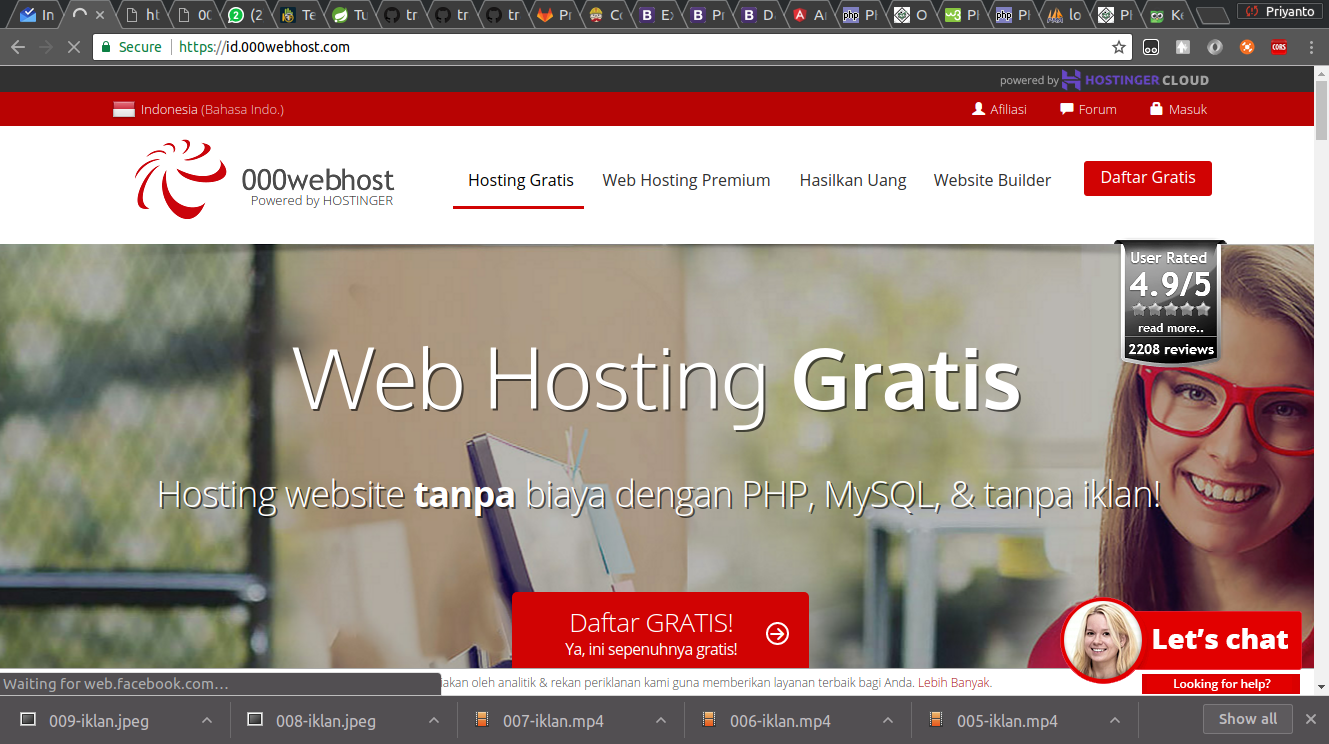
\includegraphics[width=1\textwidth]{01-03-04-001-halaman-000webhost-com}
		\caption{Tampilan Awal \textit{Website} \url{id.000webhost.com}}
		\label{fig:01-03-04-001}
	\end{figure}
	
	\item Setelah menekan tombol "Daftar Gratis", maka kemudian akan disajikan halaman seperti pada gambar \ref{fig:01-03-04-002}, kita perlu mengisikan alamat email, \textit{password} untuk masuk ke halaman manajemen \textit{website} yang kita bangun, serta alamat dari \textit{website} yang kita inginkan. Karena sifatnya gratis, \textit{url} yang disediakan pun mengikuti aturan dari penyedia \textit{hosting}.
	
	\begin{figure}[H]
		\centering
		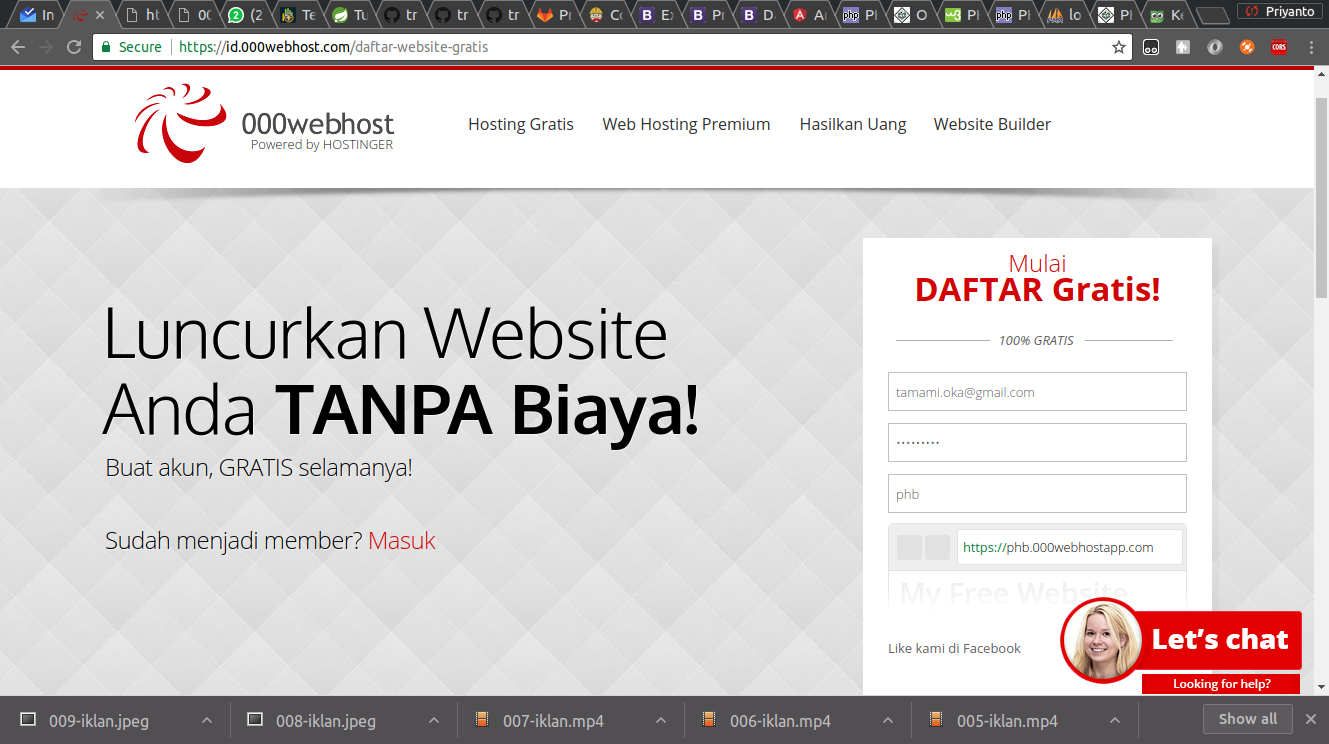
\includegraphics[width=1\textwidth]{01-03-04-002-registrasi}
		\caption{Halaman Registrasi}
		\label{fig:01-03-04-002}
	\end{figure}
	
	\item Setelah menekan tombol pendaftaran, maka akan ditampilkan halaman selamat datang seperti pada gambar \ref{fig:01-03-04-003}.
	
	\begin{figure}[H]
		\centering
		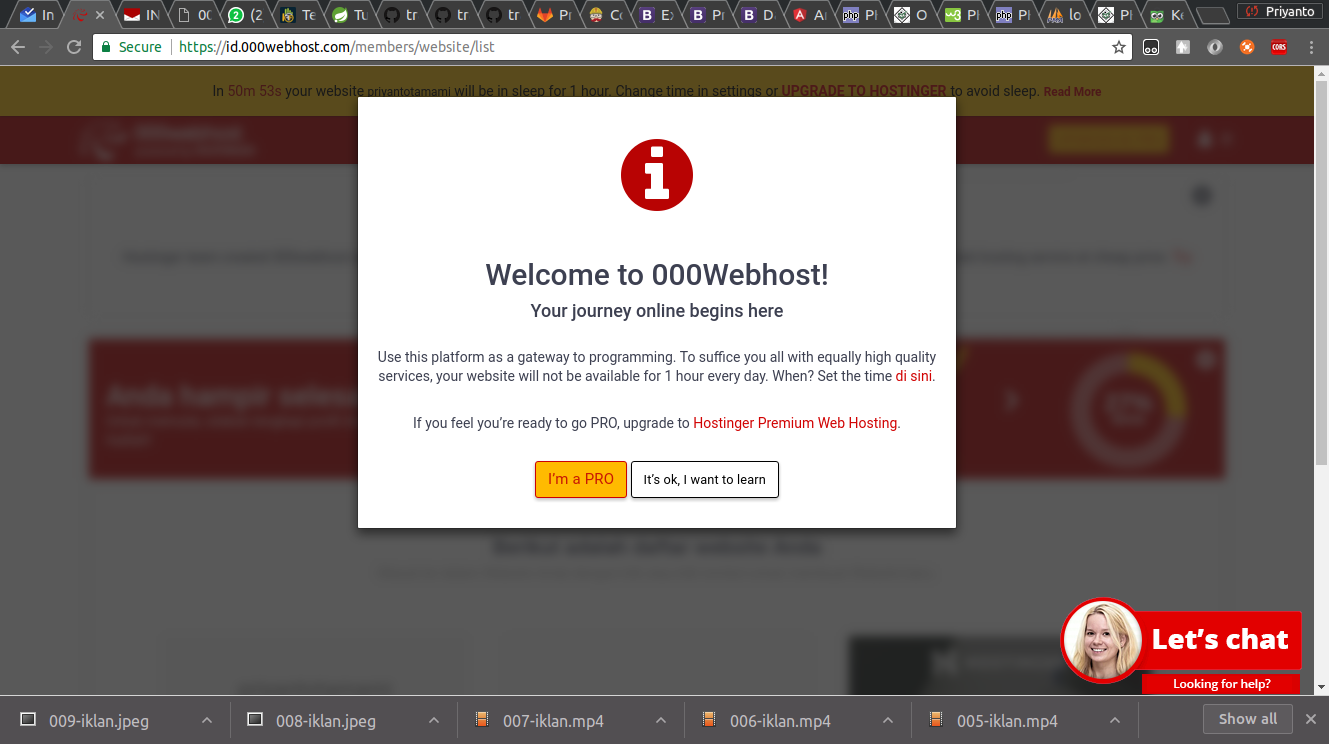
\includegraphics[width=1\textwidth]{01-03-04-003-welcome}
		\caption{Halaman Selamat Datang}
		\label{fig:01-03-04-003}
	\end{figure}
	
	\item Langkah berikutnya adalah melakukan verifikasi surel (\textit{e-mail}) seperti pada gambar \ref{fig:01-03-04-004}.
	
	\begin{figure}[H]
		\centering
		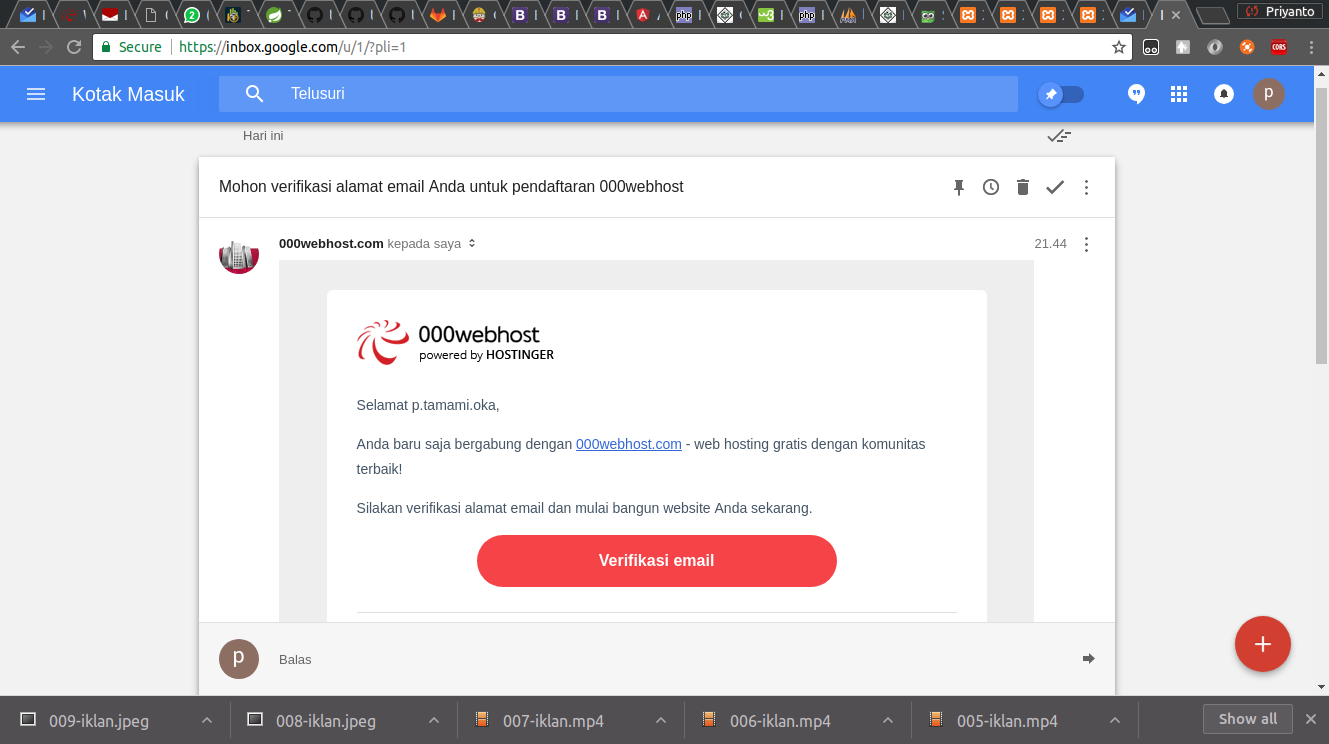
\includegraphics[width=1\textwidth]{01-03-04-004-verifikasi-email}
		\caption{Verifikasi Surel}
		\label{fig:01-03-04-004}
	\end{figure}
	
	\item Apabila verifikasi surel berhasil, maka akan tampil halaman seperti pada gambar \ref{fig:01-03-04-005}.
	
	\begin{figure}[H]
		\centering
		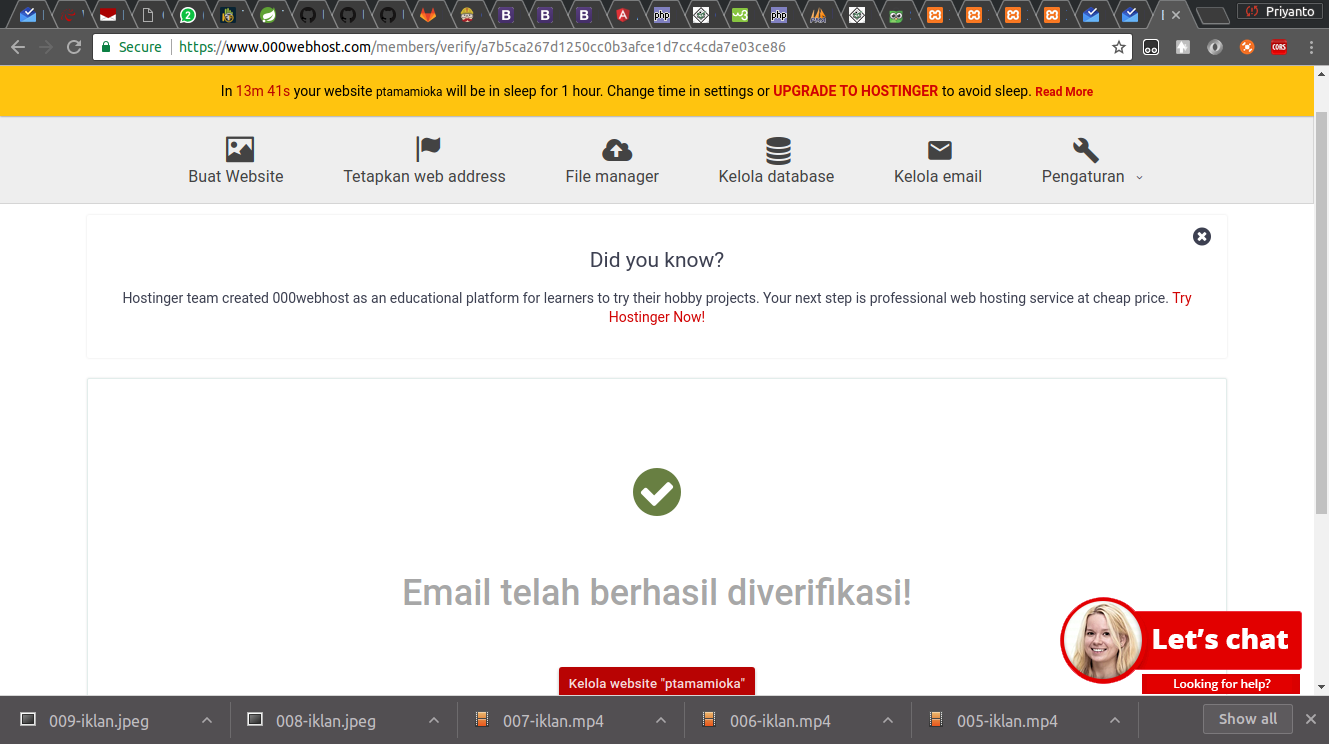
\includegraphics[width=1\textwidth]{01-03-04-005-post-verifikasi-email}
		\caption{Hasil verifikasi surel}
		\label{fig:01-03-04-005}
	\end{figure}
	
	Sampai sini, tahapan pendaftaran anggota telah berhasil kita lakukan.
	
\end{enumerate}
		
\subsection{Aplikasi Selamat Datang}

Kita akan mencoba melakukan \textit{publish} terhadap sebuah \textit{file} \texttt{html} untuk membuktikan bahwa halaman \textit{website} yang kita unggah ke \url{id.000webhost.com} dapat berhasil. Berikut adalah langkah-langkahnya :

\begin{enumerate}
	
	\item Langkah pertama adalah membuat sebuah halaman \textit{website} dengan menekan tombol kiri atas sehingga tampil halaman seperti pada gambar \ref{fig:01-03-05-001}.
	
	\begin{figure}[H]
		\centering
		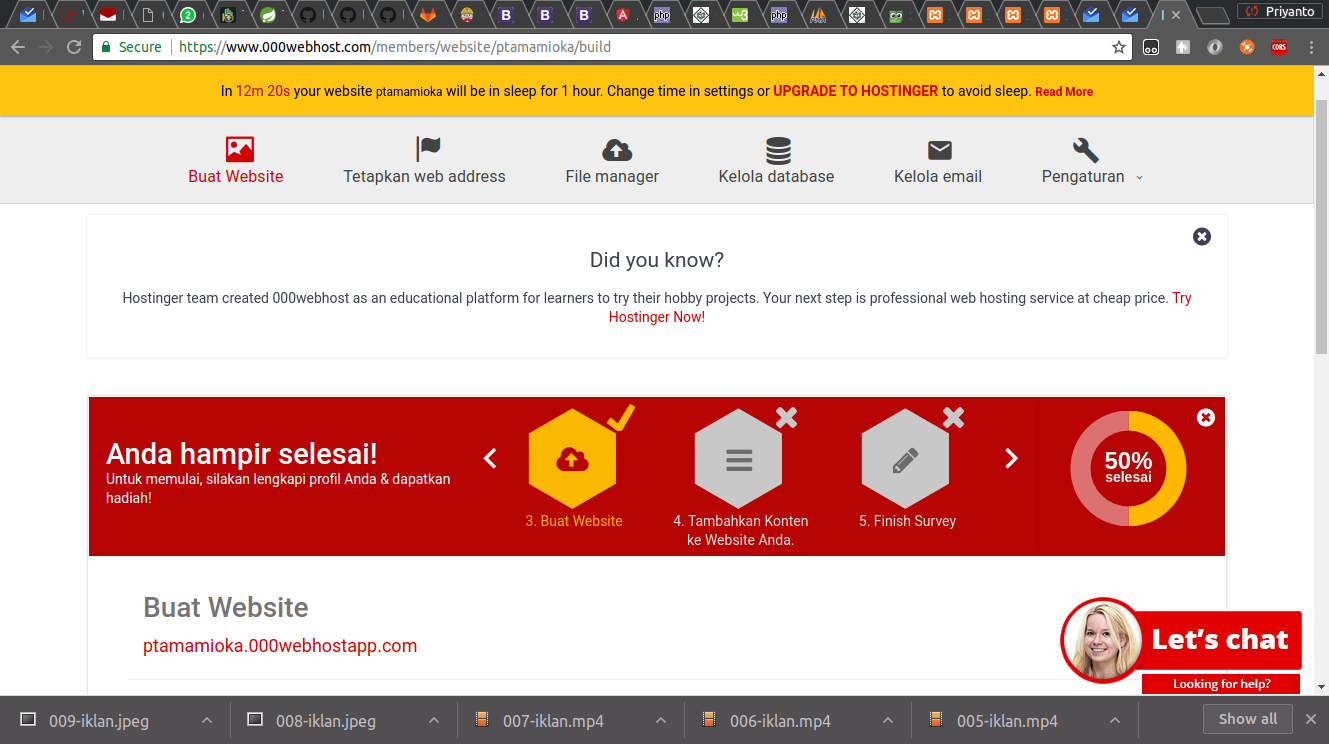
\includegraphics[width=1\textwidth]{01-03-05-001-buat-website}
		\caption{Membuat \textit{website}}
		\label{fig:01-03-05-001}
	\end{figure}
	
	\item Selanjutnya kita membuat \textit{file} dengan nama \texttt{index.html} terlebih dahulu, pembuatan \textit{file} ini dapat kita lakukan dengan notepad, vim, atau Visual Studio Code yang telah kita \textit{install}. Isi dari \textit{file} ini adalah sebagai berikut :
	
	\begin{lstlisting}[language=html]
Hai, selamat datang. \end{lstlisting}	
	
	\item Kemudian kita \textit{scroll} ke bawah halaman \url{id.000webhost.com}, maka akan muncul tampilan seperti pada gambar \ref{fig:01-03-05-003}. Karena kita telah membuat sebuah \textit{file} \texttt{index.html}, maka kita memilih "Unggah Website Sendiri".
	
	\begin{figure}[H]
		\centering
		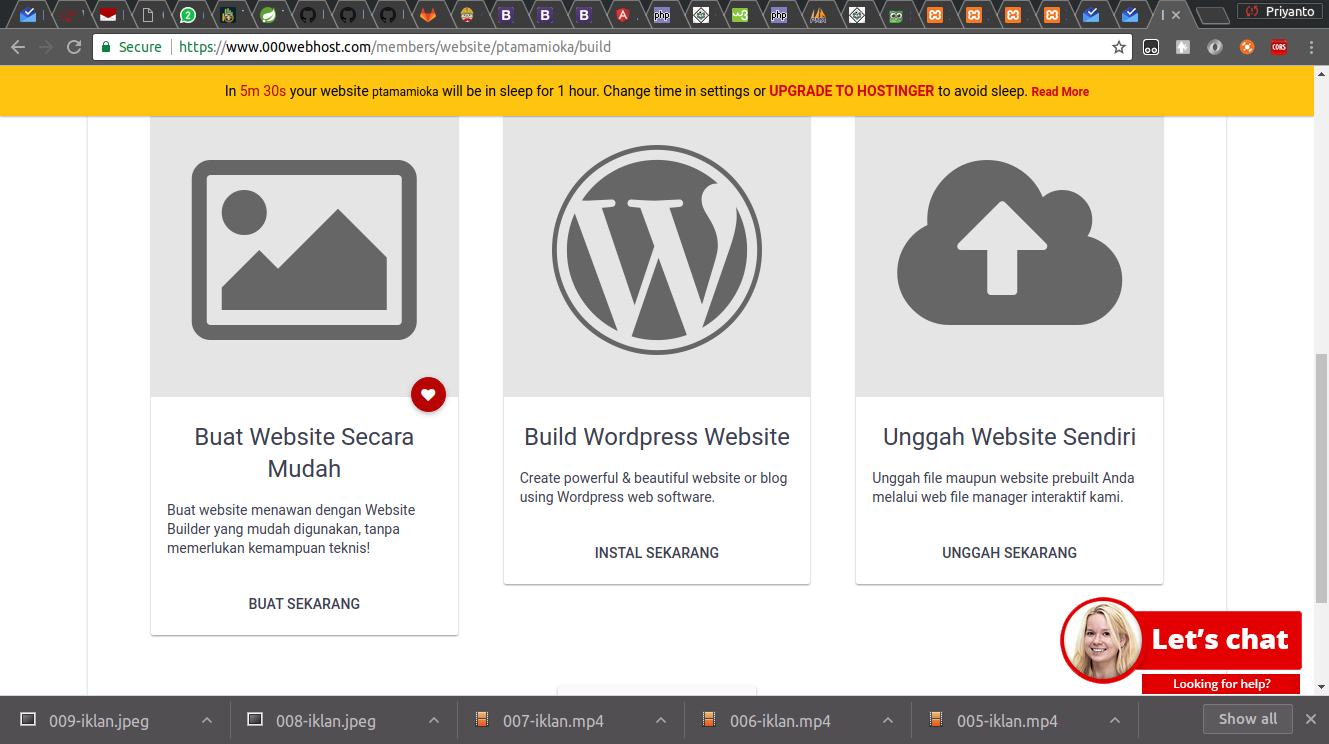
\includegraphics[width=1\textwidth]{01-03-05-003-pre-upload}
		\caption{Pilihan cara membuat \textit{website}}
		\label{fig:01-03-05-003}
	\end{figure}
	
	\item Selanjutnya kita akan ditunjukkan halaman \textit{file manager} dimana nantinya di dalam \textit{folder} \texttt{public\_html} ini \textit{project} kita ditempatkan. Tampilannya seperti pada gambar \ref{fig:01-03-05-004}.
	
	\begin{figure}[H]
		\centering
		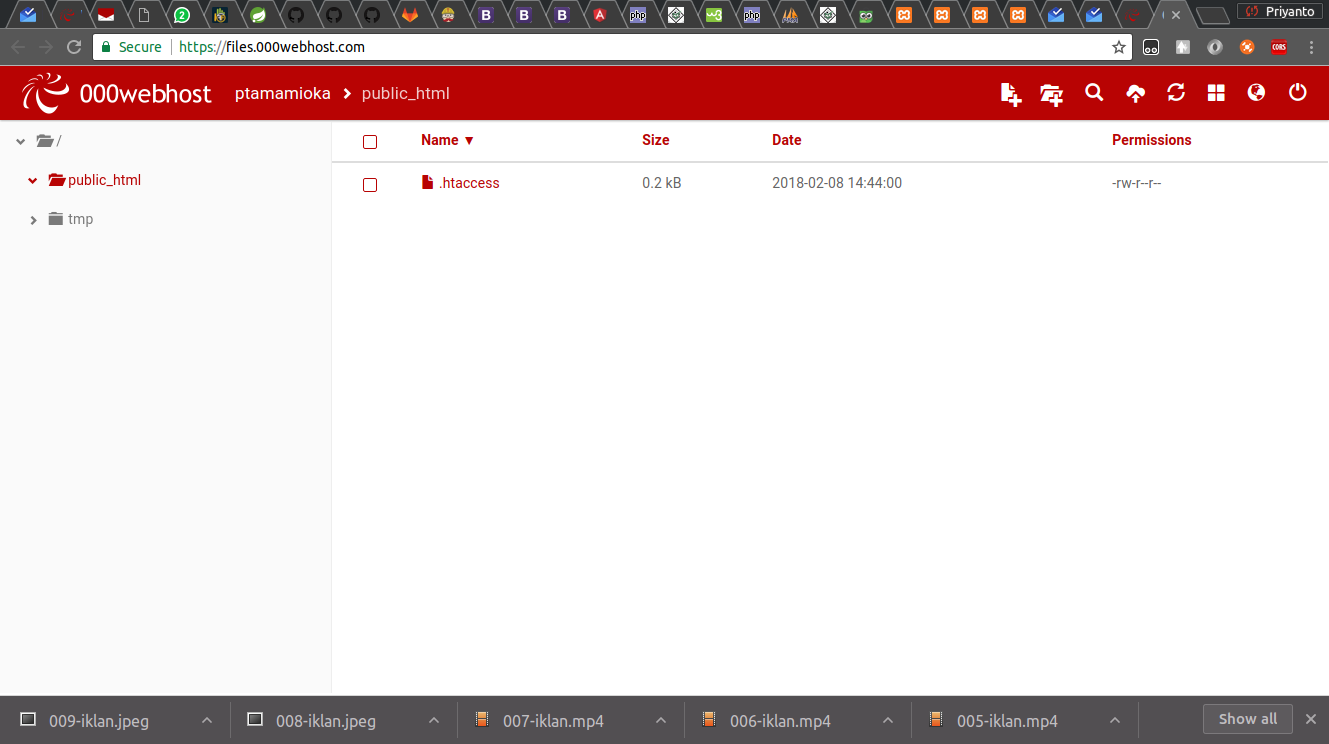
\includegraphics[width=1\textwidth]{01-03-05-004-upload}
		\caption{Halaman \textit{File Manager}}
		\label{fig:01-03-05-004}
	\end{figure}
	
	\item Pilihlah ikon dengan gambar awan dan tanda panah atas pada bagian atas kanan jendela \textit{file manager} untuk mengunggah \textit{file} \texttt{index.html} yang telah kita buat sebelumnya. Nantinya akan muncul tampilan seperti pada gambar \ref{fig:01-03-05-005}.
	
	\begin{figure}[H]
		\centering
		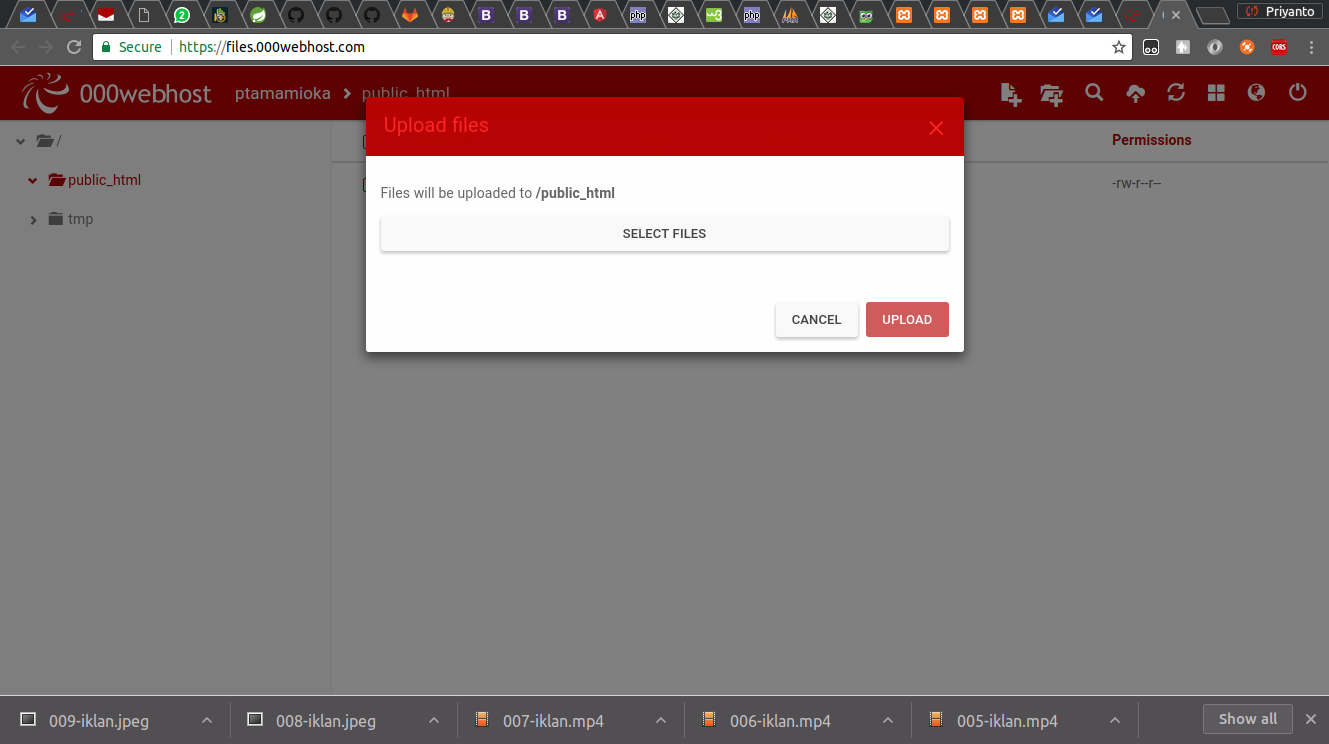
\includegraphics[width=1\textwidth]{01-03-05-005-select-files}
		\caption{Jendela Unggah \textit{File}}
		\label{fig:01-03-05-005}
	\end{figure}
	
	\item Tekanlah tombol \texttt{SELECT FILES} yang berada di tengah sehingga muncul jendela pemilihan \textit{file} seperti pada gambar \ref{fig:01-03-05-006}, lalu memilih \textit{file} dengan nama \texttt{index.html} yang akan kita unggah ke \textit{server}.
	
	\begin{figure}[H]
		\centering
		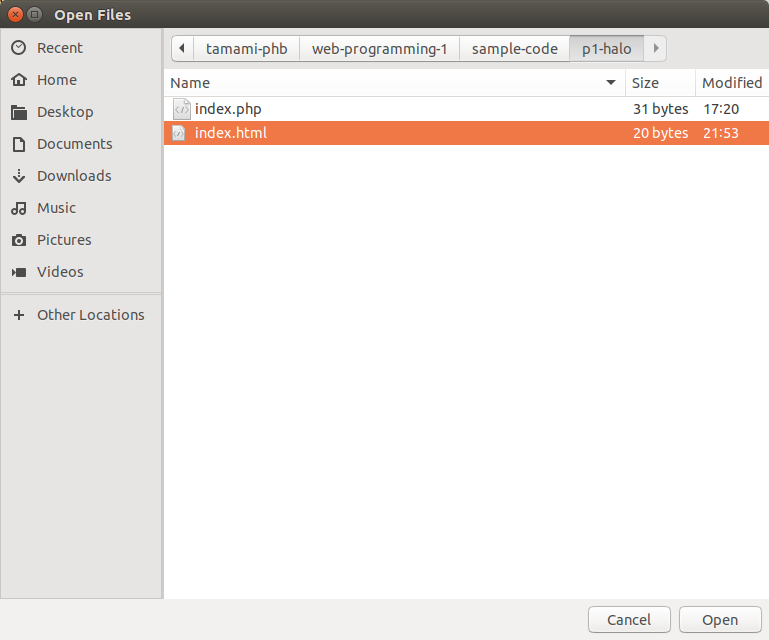
\includegraphics[width=1\textwidth]{01-03-05-006-choose-files}
		\caption{Jendela Pemilihan \textit{File}}
		\label{fig:01-03-05-006}
	\end{figure}
	
	\item Setelah \textit{file} dipilih, maka jendela \textit{Upload Files} akan menampilkan \textit{file} yang terpilih untuk selanjutnya siap diunggah seperti pada gambar \ref{fig:01-03-05-007}.
	
	\begin{figure}[H]
		\centering
		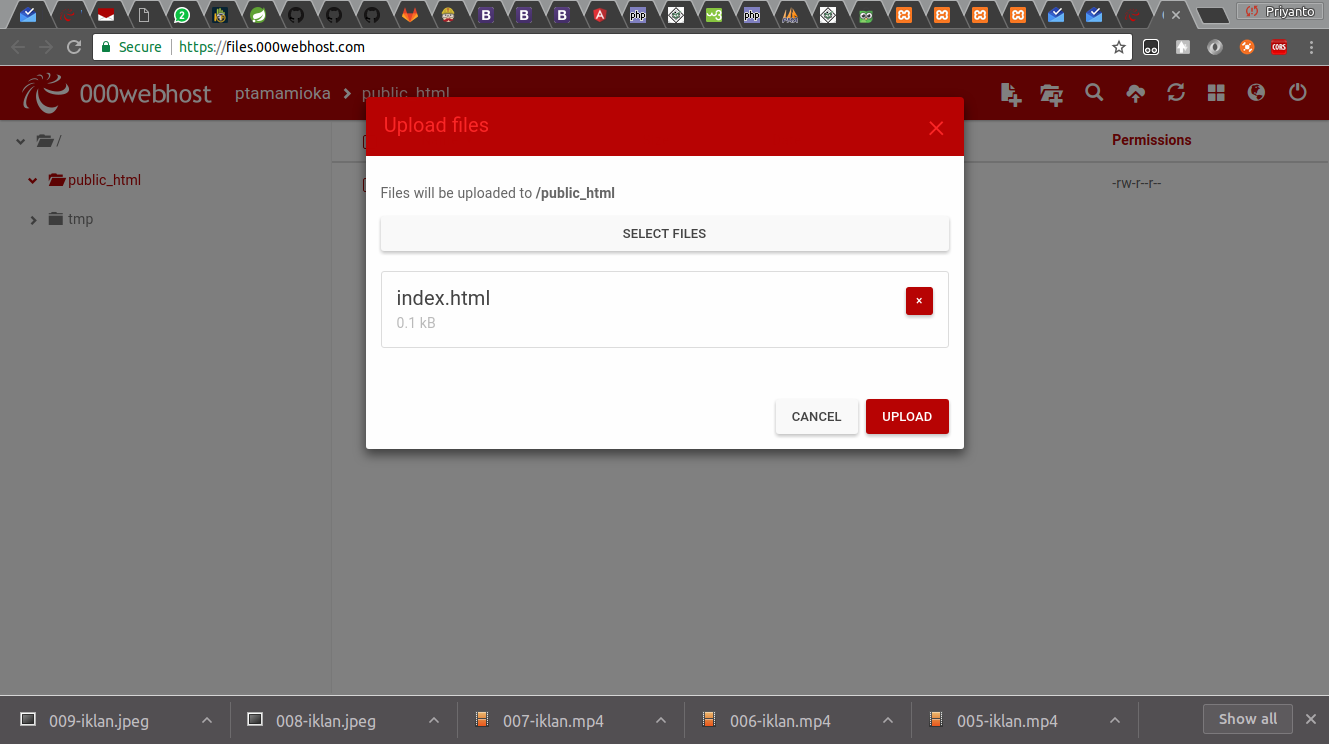
\includegraphics[width=1\textwidth]{01-03-05-007-choosen-files}
		\caption{Jendela \textit{File} Terpilih}
		\label{fig:01-03-05-007}
	\end{figure}
	
	\item Setelah selesai terunggah, maka akan tampil \textit{file} yang telah diunggah seperti pada gambar \ref{fig:01-03-05-008}. 
	
	\begin{figure}[H]
		\centering
		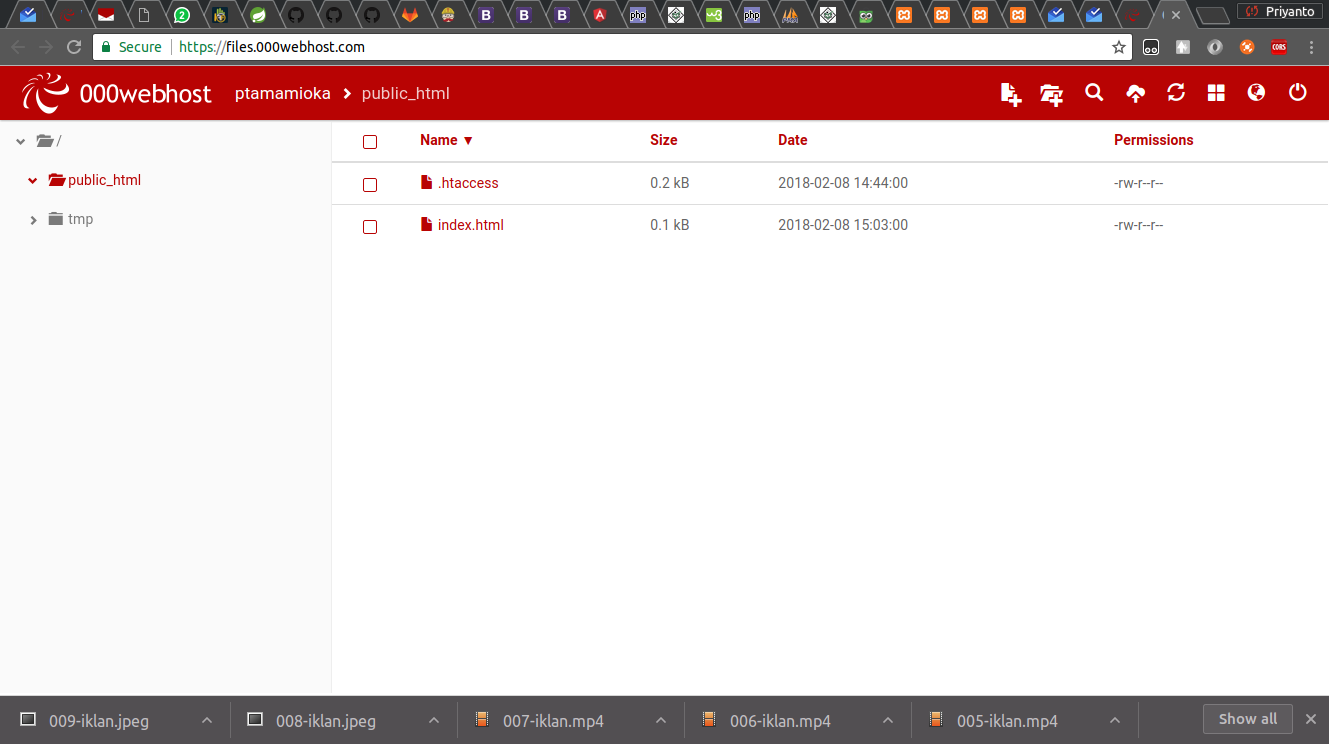
\includegraphics[width=1\textwidth]{01-03-05-008-post-upload}
		\caption{Jendela \textit{File Manager} Setelah File Terunggah}
		\label{fig:01-03-05-008}
	\end{figure}
	
	\item Lakukan akses ke halaman yang telah disediakan oleh \url{www.000webhost.com} yang hasilnya seperti terlihat pada gambar \ref{fig:01-03-05-009}. Karena ini layanan gratis, jadi jeda antara waktu \textit{file} telah terunggah dengan hasil \textit{website} memakan waktu yang bervariasi. Apabila protokol \texttt{https} tidak berhasil menampilkan halaman yang telah kita buat, cobalah menggunakan protokol \texttt{http}.
	
	\begin{figure}[H]
		\centering
		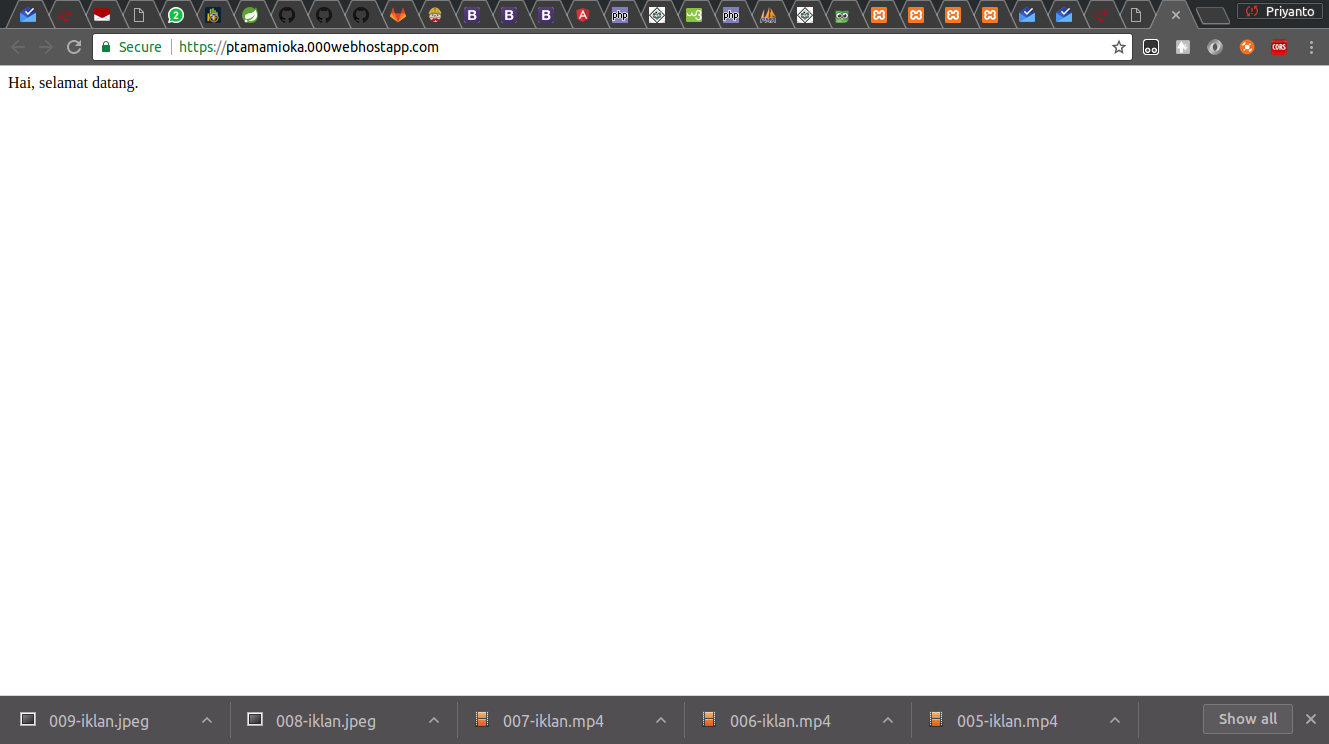
\includegraphics[width=1\textwidth]{01-03-05-009-finish}
		\caption{Hasil \textit{Website}}
		\label{fig:01-03-05-009}
	\end{figure}
	
\end{enumerate}

\subsection{Unggah ke Github}

Setelah kode awal berhasil kita unggah ke \url{id.000webhost.com}, kita akan unggah pula kode yang kita buat ke \href{github.com}{Github} untuk keperluan \textit{versioning} kode. Langkahnya cukup mudah, yaitu :

\begin{enumerate}

	\item Membuat \textit{repository} di Github dengan menekan tombol hijau bertuliskan "Create a new repository" seperti pada gambar \ref{fig:01-03-06-001}.
	
	\begin{figure}[H]
		\centering
		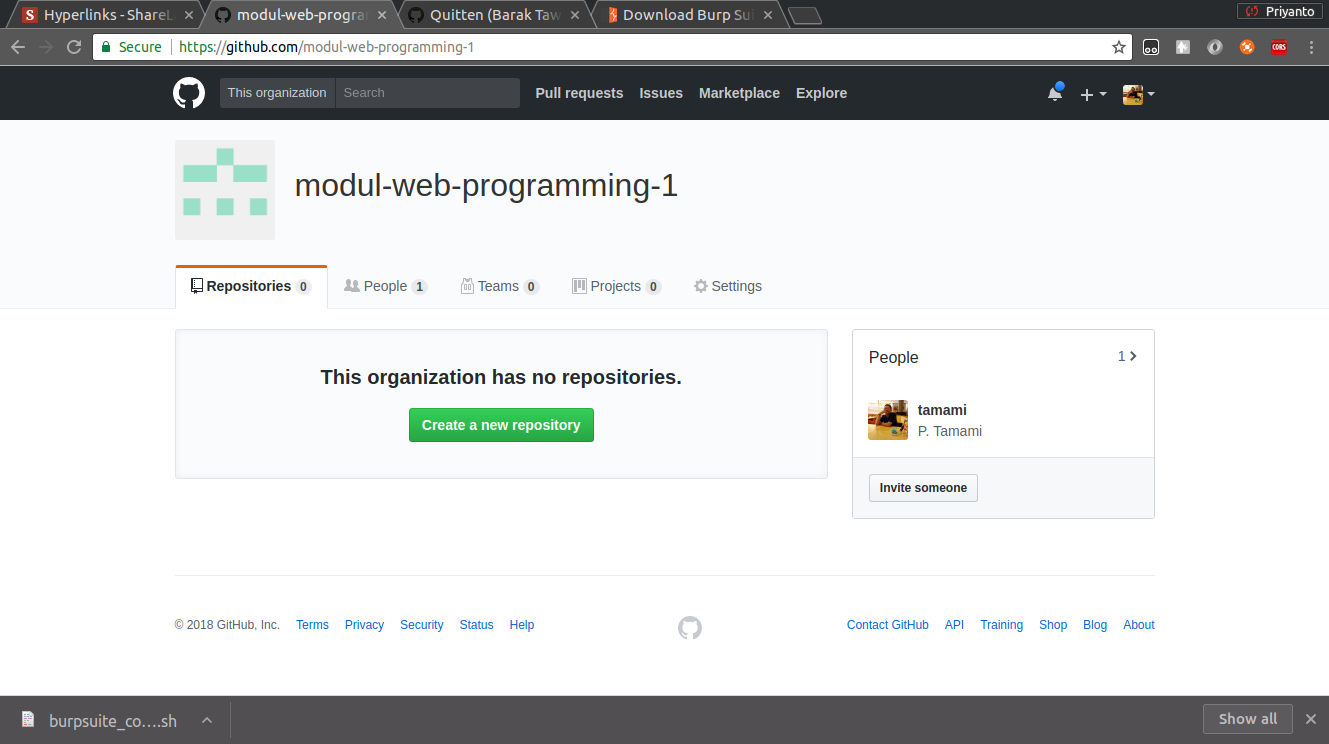
\includegraphics[width=1\textwidth]{01-03-06-001-halaman-awal-github}
		\caption{Halaman Awal Github}
		\label{fig:01-03-06-001}
	\end{figure}
	
	\item Kemudian mengisikan nama repositorinya pada kolom yang tersedia, lalu tekan tombol \texttt{Enter} atau klik tombol "Create Repository" seperti pada gambar \ref{fig:01-03-06-002} yang nantinya.
	
	\begin{figure}[H]
		\centering
		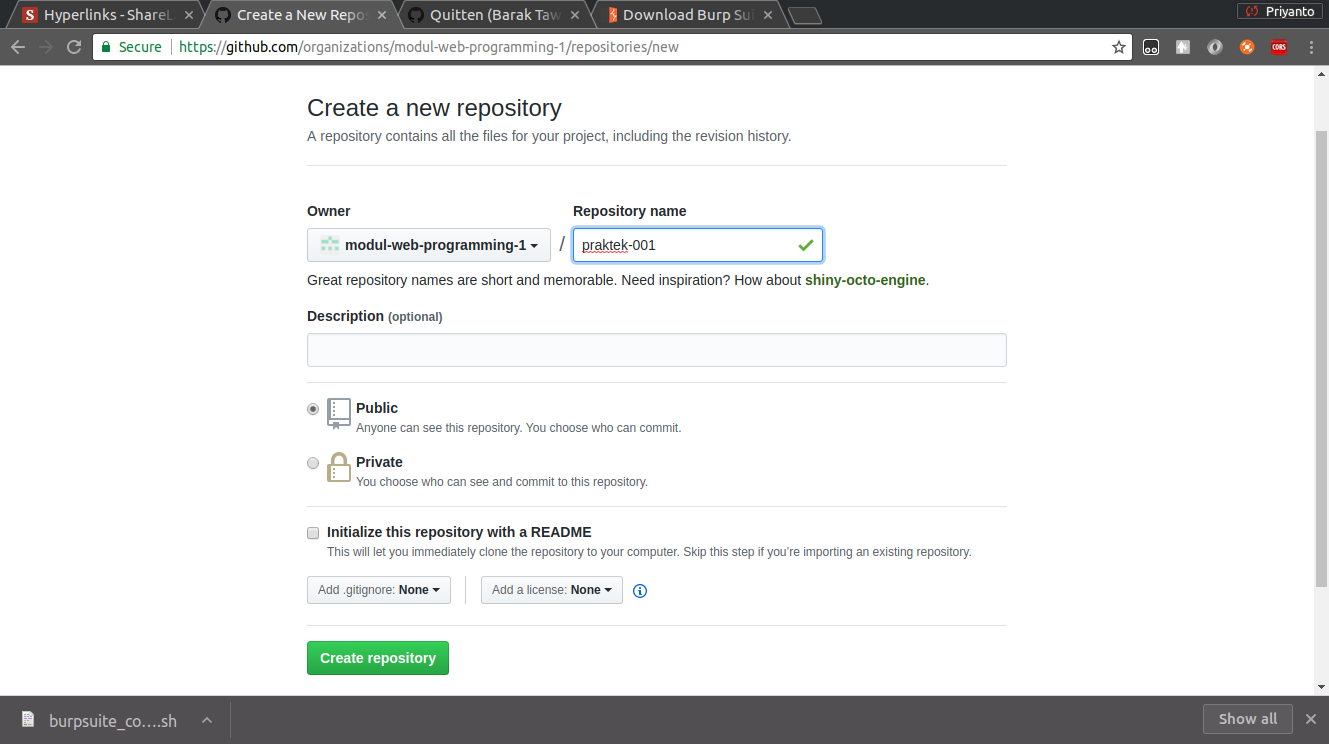
\includegraphics[width=1\textwidth]{01-03-06-002-membuat-repo}
		\caption{Membuat \textit{Repository}}
		\label{fig:01-03-06-002}
	\end{figure}
	
	\item Membuka \texttt{terminal} atau \texttt{command prompt} atau \texttt{console} untuk melakukan \textit{init} \texttt{git} dengan lokasi direktorinya adalah tempat \textit{file} \texttt{index.html} berada dengan kode berikut :
	
	\begin{lstlisting}[language=bash]
> git init	\end{lstlisting}

	\item Melakukan \textit{staging file} dengan perintah berikut :
	
	\begin{lstlisting}[language=bash]
> git add . \end{lstlisting}

	\item Melakukan \textit{commit} terhadap \textit{staging file} dengan perintah berikut :
	
	\begin{lstlisting}[language=bash]
> git commit -m "init commit" \end{lstlisting}

	Opsi perintah \texttt{-m "init commit"} sebetulnya wajib, jadi setiap kita melakukan \textit{commit}, kita diminta untuk memberikan keterangan / komentar di tiap \textit{commit} untuk memudahkan kita mencari tahap perubahan tertentu.

	\item Mendaftarkan alamat penyedia layanan repositori \texttt{git} dengan perintah berikut :
	
	\begin{lstlisting}[language=bash]
> git remote add github https://github.com/modul-web-programming-1/praktek-001.git \end{lstlisting}

	\texttt{github} di atas adalah nama alias, jadi boleh diganti apapun, sedangkan \textit{url} setelahnya adalah alamat yang diberikan oleh Github setelah kita membuat sebuah \textit{repository}.

	\item Melakukan unggah kode ke Github dengan perintah berikut :
	
	\begin{lstlisting}[language=bash]
> git push -u github master		\end{lstlisting}

	\texttt{github} adalah alias yang sebelumnya kita buat, sedangkan \texttt{master} adalah \textit{branch} utama dari \texttt{git}.
	
\end{enumerate}

\section{Kesimpulan}

Bahwa membangun sebuah aplikasi \textit{web} menggunakan PHP yang bersifat dinamis diperlukan beberapa perangkat / aplikasi pendukung.

Dengan fasilias gratis pun kita masih dapat melakukan \textit{publish project} aplikasi web yang dibangun dengan PHP kita ke internet sehingga dapat diakses oleh semua orang.

\section{Tugas}

Membuat halaman selamat datang dalam bentuk HTML dan di-\textit{publish} ke internet.